\documentclass{article}
\usepackage{parskip}
\usepackage{caption}
\usepackage{fancyhdr}
\usepackage{amsmath}
\usepackage{lastpage} 
\usepackage{hyperref}
\usepackage{graphicx} % Required for inserting images
\usepackage[margin=0.9in,top=1in,includefoot]{geometry}
\usepackage{framed} % or, "mdframed"
\usepackage[framed]{ntheorem}
\usepackage{theoremref}
\newframedtheorem{frm-thm}{Theorem}
\makeatletter
\newcommand*{\toccontents}{\@starttoc{toc}}
\newcommand{\ans}{\subsection*{Løsning}}
\makeatother


\newcommand{\RR}{\mathbb{R}}
\newcommand{\NN}{\mathbb{N}}
\newtheorem{thm}{Conjecture}

\setcounter{section}{1}

\begin{document}


\author{Ask Madsen}
\title{Løsning til mindstekravsopgaverne}
\maketitle

\toccontents
\newpage

\section*{Reduktion, procenregning og andre regneregler}

\subsubsection{Opgave 1}

Nedenfor er et udtryk reduceret.\\
\begin{align*}
    4&\cdot (5a-b)+b-3a\\
    &=20a-4b+b-3a\\
    &=17a-3b
\end{align*}
Forklar hvert trin i reduktionen\\\\

\subsubsection*{Løsning opgave 1}
I det første trin ganger vi 4 ind i parentesen på hvert led således
\begin{align*}
    4\cdot (5a-b)=4\cdot 5a - 4\cdot b=20a-4b
\end{align*}

I det næste trin samler vi ledene som indeholder a og ledene som indeholder b således
\begin{align*}
    20a -4b + b - 3a = 20a - 3a - 4b + b = 17a - 3b
\end{align*}

\newpage
\subsection{Opgave 2}

Nedenfor er en ligning løst.
\begin{align*}
    3x + 2(x+1) + 7 &= 5\\
    3x + 2x + 2 + 7 &= 5\\
    5x + 9 &= 5\\
    5x &= -4\\
    x &= -\frac{4}{5}
\end{align*}
Forklar, hvad der er gjort i hvert trin.\\\\

\ans
I det første trin ganger vi 2 tallet ind i parentesen på hvert led således 
\begin{align*}
    2(x + 1)=2x + 2
\end{align*}
I det næste trin lægger vi ledene som indeholder x sammen og ledene som ikke indeholder x sammen.
\begin{align*}
    3x + 2x +2 +7 = 5x + 9
\end{align*}
I det næste trin trækker vi 9 fra på begge sider
\begin{align*}
    5x + 9 - 9 = 5 - 9 \Longleftrightarrow 5x = -4
\end{align*}
I det sidste trin dividerer vi med 5 
\begin{align*}
    \frac{5x}{5} = -\frac{4}{5} \Longleftrightarrow x = -\frac{4}{5}
\end{align*}

\newpage
\subsection{Opgave 3}

Forklar, at værdien af $a^2 - (b+c)$ er 1, når $a = -3$, $b = 6$ og $c = 2$.\\\\

\ans
Vi starter med at indsætte værdierne for a, b og c hvorefter vi beregner parentesen og potensen og trækker så resultaterne fra hinanden
\begin{align*}
    (-3)^2 - (6 + 2) = 9 - 8 = 1
\end{align*}


\newpage
\subsubsection{Opgave 4}

Hvor mange procent udgør 30 ud af 260?\\\\

\subsubsection*{Løsning opgave 4}
For at bestemme hvor mange procent Tal1 udgør af Tal2 kan man bruge følgende formel
\begin{align*}
    \frac{Tal1}{Tal2}\cdot 100\%
\end{align*}
Hvis vi indsætter de kendte værdier Tal1$=30$ og Tal2$=260$ får vi
\begin{align*}
    \frac{30}{260}\cdot 100 \approx 11.53 \%
\end{align*}
30 udgør altså ca 11.53 \% af 260.
\vspace*{1cm}

\newpage

\section*{Løsning af ligninger}

\subsubsection{Opgave 5}

Løs følgende to ligninger med to ubekendte
\begin{align*}
   &x = 6 - y\\
    &5y + x = 14
\end{align*}

\subsubsection*{Løsning opgave 5}

Vi indsætter den første ligning $x = 6-y$ på x's plads i den anden ligning således
\begin{align*}
    5y + (6 - y) = 14
\end{align*}
I denne ligning isolerer vi så y
\begin{align*}
    &5y + (6 - y) = 14\\
    \Updownarrow \; &\\
    &5y - y + 6 = 14\\
    \Updownarrow \; &\\
    &4y + 6 = 14\\
    \Updownarrow \; &\\
    &4y = 14 - 6\\
    \Updownarrow \; &\\
    &4y = 8\\
    \Updownarrow \; &\\
    &\frac{4y}{4} = \frac{8}{4}\\
    \Updownarrow \; &\\
    &y = 2
\end{align*}
Indsætter nu $y = 2$ i den første ligning og får
\begin{align*}
    x = 6 - 2 = 4
\end{align*}
Løsningen til de 2 ligninger er derfor $x = 4$ og $y = 2$. 
\newpage
\subsubsection{Opgave 6}

Bestem diskriminanten for andengradsligningen
\begin{align*}
    3x^2 + 4x -1 = 0
\end{align*}

\subsubsection*{Løsning opgave 6}

Den generelle formel for diskriminanten er $d = b^2 - 4\cdot a\cdot c$. Vi ved at den generelle andengradsligning skrives på formen $ax^2 + bx + c = 0$. Vi aflæser nu a, b og c og får følgende $a = 3,\; b = 4,\; c = -1$. Diskriminanten bliver dermed
\begin{align*}
    d = 4^2 -4\cdot 3\cdot (-1) = 16 - (-12) = 16 + 12 = 28
\end{align*}
\newpage
\subsubsection*{Opgave 7}

Løs denne ligning: $\cfrac{20}{x+2} = 4$\\\\

\subsubsection*{Løsning opgave 7}
Vi starter med at dividere med 20 på begge sider
\begin{align*}
    \frac{20}{20(x+2)}=\frac{4}{20} \Longrightarrow \frac{1}{x+2} = \frac{4}{20}
\end{align*}
Nu kan vi bytte om på tæller og nævner på begge sider af lighedstegne så vi får
\begin{align*}
    x+2 = \frac{20}{4}
\end{align*}
Nu trækker vi 2 fra på begge sider og får
\begin{align*}
    x + 2 - 2 = \frac{20}{4}- 2
\end{align*}
Ved at omskrive 2 tallet til $2 = \frac{8}{4}$ får vi nu
\begin{align*}
    x = \frac{20}{4}-\frac{8}{4}=\frac{20-8}{4}=\frac{12}{4}=3
\end{align*}
\newpage
\subsubsection{Opgave 8}

Undersøg om $x = 2$ er en løsning til denne ligning: $x^2 -5x + 6 = 0$.\\\\

\subsubsection*{Løsning opgave 8}

For at undersøge om $x = 2$ er en løsning til ligningen indsætter vi 2 på x's plads og ser om venstresiden giver 0.
\begin{align*}
    2^2 -5\cdot 2 + 6 = 4 - 10 + 6 = 10 - 10 = 0
\end{align*}
$x = 2$ er altså en løsning til ligningen. 
\newpage
\subsection{Opgave 9}

To linjer er givet ved $y = 4x -1$ og $y = x  + 5$. Bestem skæringspunktet mellem de to linjer.\\\\


\ans
For at bestemme skæringspunktets x-koordinat mellem de to linjer kan vi sætte dem lig med hinanden og isolere for x.
\begin{align*}
    &4x -1 = x + 5\\
    \Updownarrow \; &\\
    &4x -1 + 1 = x + 5 + 1\\
    \Updownarrow \; &\\
    &4x = x + 6\\
    \Updownarrow \; &\\
    &4x - x = x - x + 6\\
    \Updownarrow \; &\\
    &3x = 6\\
    \Updownarrow \; &\\
    &\frac{3x}{3} = \frac{6}{3}\\
    \Updownarrow \; &\\
    &x = 2
\end{align*}
Herefter indsætter vi $x = 2$ i en af de to linjers forskrift og bestemmer skæringspunktets y-koordinat
\begin{align*}
    y = 2 + 5 = 7
\end{align*}
Skæringspunktet mellem de to linjer er derfor $(2,7)$
\newpage
\subsection{Opgave 10}

Isolér $T$ i ligningen $a\cdot T = \frac{R-T}{Q+a}$.\\\\

\ans
Vi starter med at gange med $(Q+a)$ på begge sider
\begin{align*}
    a\cdot T \cdot (Q+a) = \frac{R-T}{Q+a}\cdot (Q+a) \Longrightarrow aQT + a^2T = R-T
\end{align*}
Vi lægger nu $T$ til på begge sider
\begin{align*}
    aQT + a^2T + T = R 
\end{align*}
Nu sætter vi $T$ uden for en parentes så $(aQ + a^2 + 1)T = aQT + a^2T + T$
\begin{align*}
    (aQ + a^2 + 1)T = R
\end{align*}
Dividerer nu med $(aQ + a^2 + 1)$ på begge sider og får
\begin{align*}
    T = \frac{R}{aQ + a^2 + 1}
\end{align*}
$T$ er hermed isoleret i ligningen.

\section*{Geometri og trigonometri}

\subsection{Opgave 11}
Figuren viser en trekant $ABC$.\\\\
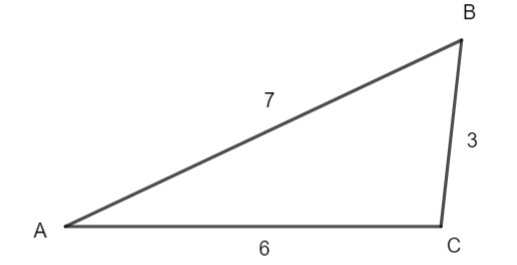
\includegraphics[width=10cm]{Opgave_11-20/Opgave_11/Opgave_11.jpg}

Følgende sidelængder er kendte: $|AB| = 7,\; |BC| = 3$ og  $|AC| = 6$.\\\\
Bestem vinkel $A$.\\\\


\ans
Da trekanten ikke er retvinkel kan vi bruge cosinusrelationen
\begin{align*}
    a^2 = b^2 + c^2 -2\cdot b\cdot c\cdot \cos(A)
\end{align*}
Her isolerer vi først cos(A)
\begin{align*}
    &a^2 -b^2 - c^2 = -2\cdot b\cdot c\cdot \cos(A)\\
    \Updownarrow \; &\\
    &\frac{a^2 - b^2 - c^2}{-2\cdot b\cdot c} = \cos(A)\\
    \Updownarrow \; &\\
    &-\frac{a^2 - b^2 - c^2}{2\cdot b\cdot c} = \cos(A)
\end{align*}
Nu indsætter vi sidelængderne på a,b og c's plads så $a = 3,\; b = 6$ og $c = 7$
\begin{align*}
    &-\frac{3^2 - 6^2 - 7^2}{2\cdot 6\cdot 7} = \cos(A)\\
    \Updownarrow \; &\\
    &-\frac{9 - 36 - 49}{84} = \cos(A)\\
    \Updownarrow \; &\\
    &-\frac{-76}{84} =  \cos(A)\\
    \Updownarrow \; &\\
    &\frac{76}{84} = \cos(A)\\
\end{align*}
Nu bruger vi den inverse funktion til cos altså arccos for at bestemme vinklen A
\begin{align*}
    A = \arccos\left(\frac{76}{84}\right) \approx 25.2 ^{\circ}
\end{align*}
\newpage
\subsection{Opgave 12}
To ensvinklede trekanter er vist på figuren.\\\\
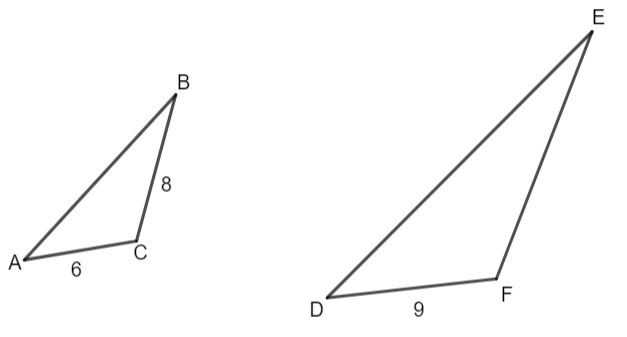
\includegraphics[width=10cm]{Opgave_11-20/Opgave_12/Opgave_12.jpg}\\\\
\textbf{Størrelsesforholdene er ikke korrekte.}\\\\

Følgende sidelængder oplyses: $|AC| = 6,\; |BC| = 8$ og $|DF| = 9$\\\\

Bestem $FE|$\\\\

\ans
Da trekanterne er ensvinklede kan vi altså bestemme sidelængdernes størrelsesforhold. Hvis vi ser på sidelængderne $|AC|$ og $|DF|$ er den større trekants side 1.5 gange længere. Vi kan altså bestemme sidelængden $|FE| = 1.5\cdot |BC| = 1.5\cdot 8 = 12$. 
\newpage
\subsection{Opgave 13}

Figuren viser en trekant\\\\
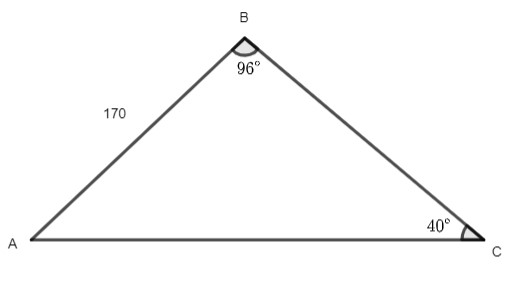
\includegraphics[width=10cm]{Opgave_11-20/Opgave_13/Opgave_13.jpg}\\\\
Følgende størrelser i trekant $ABC$ er kendte:\\\\
$B = 96^{\circ},\quad |AB| = 170\quad \text{og}\quad C = 40^{\circ}$\\\\

Bestem $|AC|$.\\\\

\ans
For at bestemme længden af siden $AC$ bruger vi sinusrelationen for en vilkårlig trekant
\begin{align*}
    \frac{a}{\sin(A)} = \frac{b}{\sin(B)} = \frac{c}{\sin(C)}
\end{align*}
Her svarer sidelængen $AB$ til c og sidelængden $AC$ som vi skal finde svarer til b. Vi betragter den sidste lighed i sinusrelationen og isolerer b.
\begin{align*}
    \frac{b}{\sin(B)} =\frac{c}{\sin(C)} \Longleftrightarrow b = \frac{c}{\sin(C)}\cdot \sin(B)
\end{align*}
Indsætter nu $c = 170,\quad C = 40^{\circ},\quad B = 96^{\circ}$ og får 
\begin{align*}
    b = \frac{170}{\sin(40^{\circ})}\cdot \sin(96^{\circ})\approx 263.03
\end{align*}
\newpage
\subsection{Opgave 14}

En retvinklet trekant er skitseret på figuren.\\\\
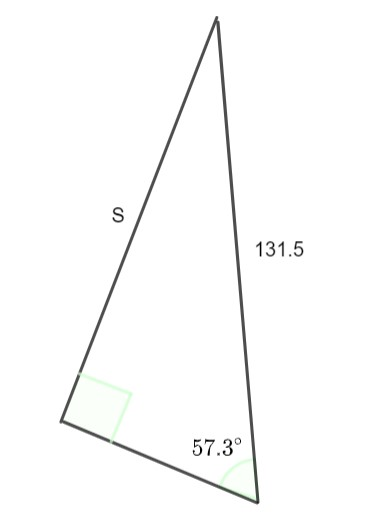
\includegraphics[width=7cm]{Opgave_11-20/Opgave_14/Opgave_14.jpg}\\\\
Bestem længden S.\\\\

\ans
For retvinklede trekanter gælder formlen
\begin{align*}
    \sin(B) = \frac{c}{b}
\end{align*}
Her er B vinklen $B = 57.3^{\circ}$, c er længden af hypotinusen dvd $c = 131.5$ og b er siden som i vores tilfælde svarer til s. Vi isolerer altså b og indsætter tallene
\begin{align*}
    \sin(B) = \frac{b}{c} \Longleftrightarrow b = \sin(B)\cdot c = \sin(57.3^{\circ})\cdot 131.5 \approx 89.76
\end{align*}

\newpage
\subsection{Opgave 15}

Et punkt har koordinatsættet $A(8,6)$.\\\\
En linje $l$ har ligningen $y = -x+7$.\\\\
Bestem afstanden mellem $A$ og $l$.\\\\

\ans
Her bruger vi formlen for afstand mellem et punkt og en linje som siger at afstanden fra et punkt $(x_1,y_1)$ til en linje $y = ax+b$ kan bestemmes ved
\begin{align*}
    \text{dist}(P,m)=\frac{|ax_1+b-y_1|}{\sqrt{a^2 +1}}
\end{align*}
Vi indsætter tallene og får
\begin{align*}
    \text{dist}(P,m)=\frac{|(-1)\cdot 8+7-6|}{\sqrt{(-1)^2 + 1}}= \frac{|-8+1|}{\sqrt{1+1}}=\frac{|-7|}{\sqrt{2}}=\frac{7}{\sqrt{2}}\approx 4.95
\end{align*}
\newpage
\subsection{Opgave 16}

En cirkel $C$ og en linje $l$ er bestemt ved ligningerne
\begin{align*}
    C&:(x-4)^2 + (y-5)^2 = 3^2\\
    l&:y = x-2
\end{align*}
 a) Tegn cirklen og linjen i samme koordinatsystem.\\

 \ans
 Vi starter med at aflæse cirklens centrumskoordinat og cirklens radius. Vi ved at cirklens generelle ligning er givet ved
 \begin{align*}
     (x-a)^2 + (y-b)^2 = r^2
 \end{align*}
 Her er $C(a,b)$ cirklens centrumskoordinat og r er cirklens radius. Hvis vi bruger dette kan vi aflæse centrumskoordinatet til $C(4,5)$ og radius til $r = 3$. Vi kan nu indtegne cirklen i et koordinatsystem\\\\
 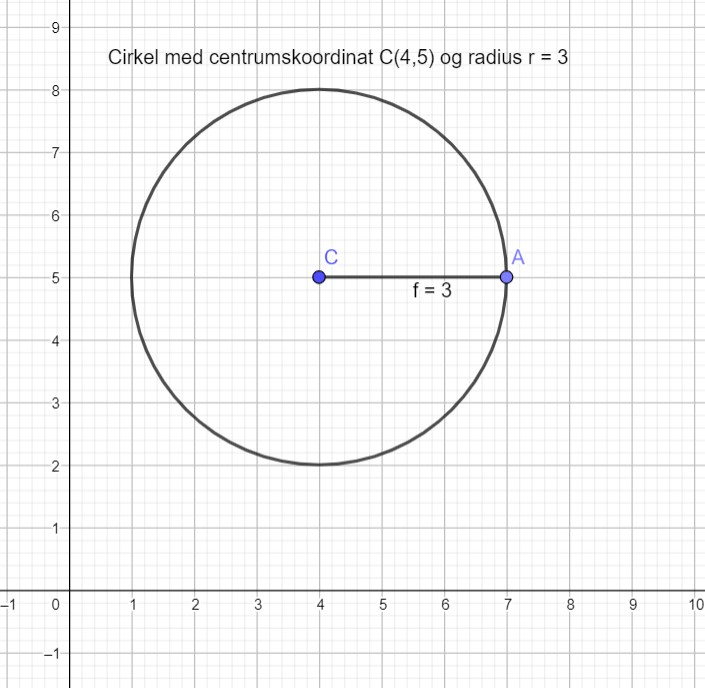
\includegraphics[width=8cm]{Opgave_11-20/Opgave_16/16.jpg}\\\\
 
 For at indtegne linjen skal vi aflæse linjens hældning, a og linjens skærings med y-aksen, b. Vi ved at en ret linje har den generelle form
 \begin{align*}
     y = ax+b
 \end{align*}
 Aflæser vi nu den givne linje får vi hældningen $a = 1$ og skæringen med y-aksen $b = -2$. Ud fra disse oplysninger kan vi nu indtegne vores linje i koordinatsystemet\\\\
 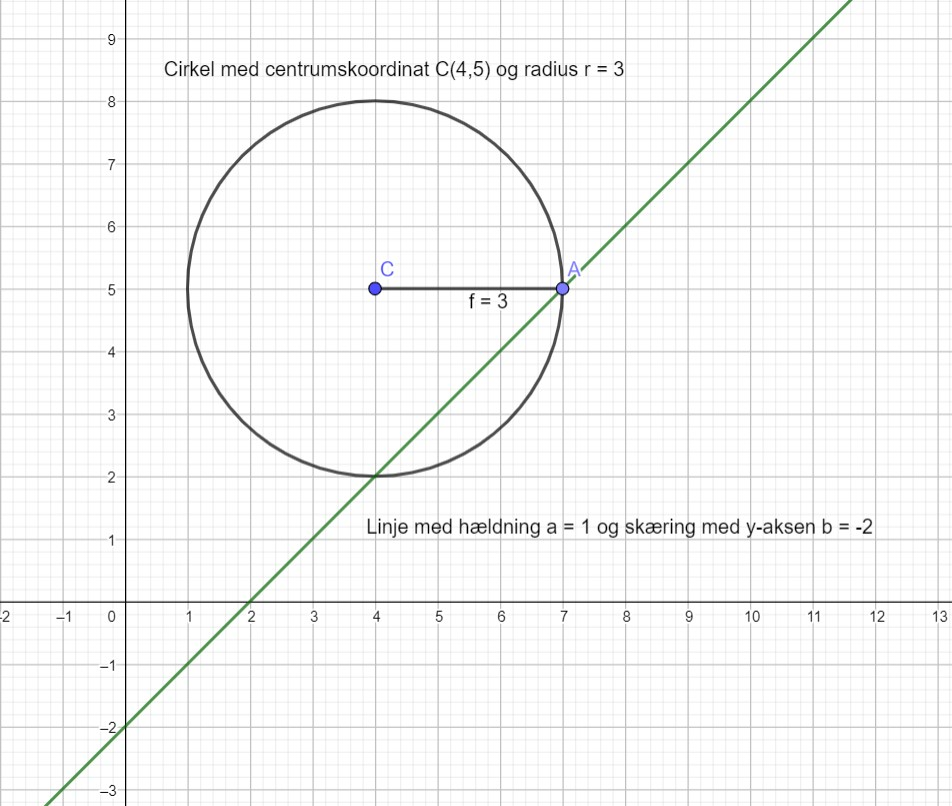
\includegraphics[width = 8cm]{Opgave_11-20/Opgave_16/16.1.jpg}\\\\
 
 b) Bestem skæringspunkterne mellem cirklen og linjen\\\\

 \ans
 
 Ud fra koordinatsystemet i opgave 16a kan vi se at cirklen og linjen skærer hinanden i 2 punkter. For at bestemme disse skæringspunkter sætter vi linjens ligning $y = x-2$ ind på y's plads i cirklens ligning
 \begin{align*}
     &(x-4)^2 + (x-2-5)^2 = 3^2\\
     \; \Updownarrow &\\
     &(x-4)^2 + (x-7)^2 = 9\\
 \end{align*}
 Vi beregner nu de 2 parenteser ved at bruge reglen $(a-b)^2 = a^2+2\cdot a\cdot (-b) + (-b)^2$
 \begin{align*}
     (x-4)^2 = x^2 +2\cdot x \cdot (-4) + (-4)^2 = x^2 -8x + 16\\
     (x-7)^2 = x^2 +2\cdot x \cdot (-7) + (-7)^2 = x^2 -14x + 49
 \end{align*}
 Indsætter vi dette får vi nu
 \begin{align*}
    &(x-4)^2 + (x-7)^2 = 9\\
    \; \Updownarrow &\\ 
    &x^2-8x+16+x^2-14x+49 = 9\\
    \; \Updownarrow &\\
    &x^2+x^2 -8x - 14x + 16+49=9\\
    \; \Updownarrow &\\
    &2x^2 - 22x + 65 = 9
 \end{align*}
 Vi trækker nu 9 fra på begge sider 
 \begin{align*}
     &2x^2 -22x +65-9 = 9-9\\
     \; \Updownarrow &\\
     &2x^2 -22x 56 = 0
 \end{align*}
 Nu findes vi løsningerne til det ovenstående andengradsligning ved først at beregne determinanten 
 \begin{align*}
     d = b^2 -4ac = (-22)^2 -4\cdot 2\cdot 56 = 36
 \end{align*}
 Nu bestemmer vi løsningerne altså x-koordinatet til skæringen mellem cirklen og linjen
 \begin{align*}
     x_1 = \frac{-b+\sqrt{d}}{2a}=\frac{22+\sqrt{36}}{2\cdot 2}=\frac{22+6}{4}=\frac{28}{4}=7\\
     x_2 = \frac{-b-\sqrt{d}}{2a}=\frac{22-\sqrt{36}}{2\cdot 2}=\frac{22-6}{4}=\frac{16}{4} = 4
 \end{align*}
 For at finde de tilsvarende skæringer med y-aksen indsætter vi de fundne x-værdier i linjens ligning
 \begin{align*}
     y_1 = x_1 -2 = 7-2 = 5\\
     y-2 = x_2 -2 = 4-2 = 2
 \end{align*}
 Vi har altså føgende skæringspunkter mellem linjen og cirklen
 \begin{align*}
     S_1=(x_1, y_1)=(7,5)\\
     S_2 =(x_2,y_2)=(4,2)
 \end{align*}
 Hvis vi sammenligner med tegningen vi får fra opgave 16a kan vi se at skærngspunkterne stemmer.
\newpage
\subsection{Opgave 17}

En cirkel $C$ er givet ved ligningen
\begin{align*}
    C:(x-2)^2 + (y-3)^2 = 5^2
\end{align*}
Bestem cirklens centrum og radius\\\\

\ans

Hvis vi benytter os af den generelle formel for cirklens ligning fra opgave 16 kan vi aflæse cirklens centrum til $C(2,3)$ og cirklens radius til $r = 5$

\newpage
\subsection{Opgave 18}

Undersøg om punktet $(2,3)$ ligger på linjen bestemt ved $2x + y - 7 = 0$\\\\

\ans
For at tjekke om et punkt ligger på en bestemt linje indsætter vi punktets x-koordinat på x'plads og punktets y-koordinat på y's plads.
\begin{align*}
    2\cdot 2 + 3 - 7 = 4 + 3 -7 = 7-7 =0
\end{align*}

Da venstresiden af vores beregning stemmer med højresiden altså 0 kan vi konkludere at punktet $(2,3)$ ligger på linjen.
\newpage
\subsection{Opgave 19}

På figuren ses en linje i et koordinatsystem.\\\\
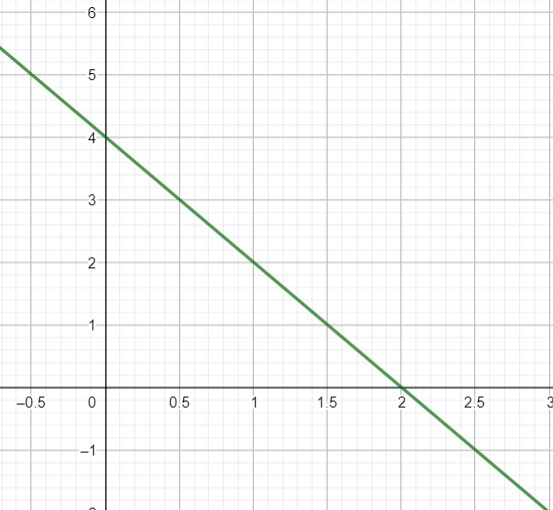
\includegraphics[width=8cm]{Opgave_11-20/Opgave_19/19.jpg}\\\\
Bestem en ligning for linjen.\\\\

\ans
Vi ved at en linje som denne har den generelle form $y = ax + b$. Her er a hældningen og b er skæringen med y-aksen. Vi aflæser skæringen med y-aksen på grafen til $b = 4$. For at bestemme hældningen $a$ skal vi benytte os af følgende formel
\begin{align*}
    a = \frac{y_2-y_1}{x_2-x_1}
\end{align*}
Her er $(x_1,y_1)$ og $(x_2,y_2)$ to vilkårlige punkter på vores linje. For nemhedens skyld vælger vi punkterne til at være 
\begin{align*}
    (x_1,y_1) = (0,4)\\
    (x_2,y_2) = (2,0)
\end{align*}
Indsætter vi disse punkter i formlen bestemmer vi nu a
\begin{align*}
    a = \frac{0-4}{2-0}=\frac{-4}{2}=-2
\end{align*}
Linjens ligning er derfor
\begin{align*}
    y = -2x + 4
\end{align*}

\section*{Vektorer}

\subsection{Opgave 20}

En vektor $\Vec{a}$ er bestemt ved
\begin{align*}
    \Vec{a} = \begin{pmatrix}-1 \\ 4\end{pmatrix}
\end{align*}
Indtegn vektoren i et koordinatsystem, og bestem $|\Vec{a}|$\\\\

\ans
Hvis vi lader vores vektor starte i punktet (0,0) så fortæller vektorens koordinater os at vi skal bevæge os -1 hen ad x-aksen og 4 op ad y-aksen. Forbinder vi disse punkter og tegner en pil op for enden af stregen får vi følgende graf\\\\
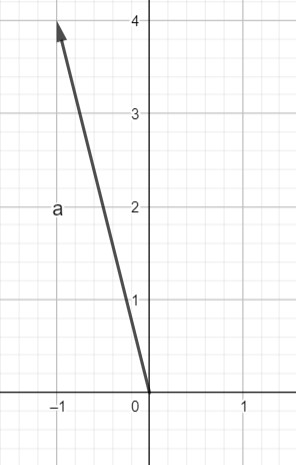
\includegraphics[width = 6cm]{Opgave_11-20/Opgave_20/20.jpg}
\newpage
\subsection{Opgave 21}

To vektorer $\Vec{a}$ og $\Vec{b}$ er givet ved
\begin{align*}
    \Vec{a} = \begin{pmatrix}-3 \\ 4\end{pmatrix}\; \text{og}\; \Vec{b} = \begin{pmatrix}1 \\ 3\end{pmatrix}
\end{align*}
Bestem vektor $\Vec{c}$, når $\Vec{c} = \Vec{a}+2\Vec{b}$\\\\

\ans
Vi kan bestemme vektor c bed følgende
\begin{align*}
    \Vec{c} = \Vec{a} + 2\Vec{b} = \begin{pmatrix}-3 \\ 4\end{pmatrix} + 2\begin{pmatrix}1 \\ 3\end{pmatrix}=\begin{pmatrix}-3 \\ 4\end{pmatrix} + \begin{pmatrix}2\cdot 1 \\ 2\cdot 3\end{pmatrix}=\begin{pmatrix}-3 \\ 4\end{pmatrix} + \begin{pmatrix}2 \\ 6\end{pmatrix}=\begin{pmatrix}-3+2 \\ 4+6\end{pmatrix} = \begin{pmatrix}-1 \\ 10 \end{pmatrix} 
\end{align*}
\newpage
\subsection{Opgave 22}

En vektor $\Vec{a}$ er bestemt ved
\begin{align*}
    \Vec{a} = \begin{pmatrix}5\cdot \cos(60^{\circ}) \\ 5\cdot \sin(60^{\circ})\end{pmatrix}
\end{align*}
Forklar hvad tallene 5 og $60^{\circ}$ fortæller om $\Vec{a}$\\\\

\ans
Tallet 5 fortæller os at $\Vec{a}$ har længden 5. Tallet $60^{\circ}$ er vektorens retningsvinkel altså den vinkel der er mellem vektoren og x-aksen. Dette kan ses illustreret på følgende graf\\\\
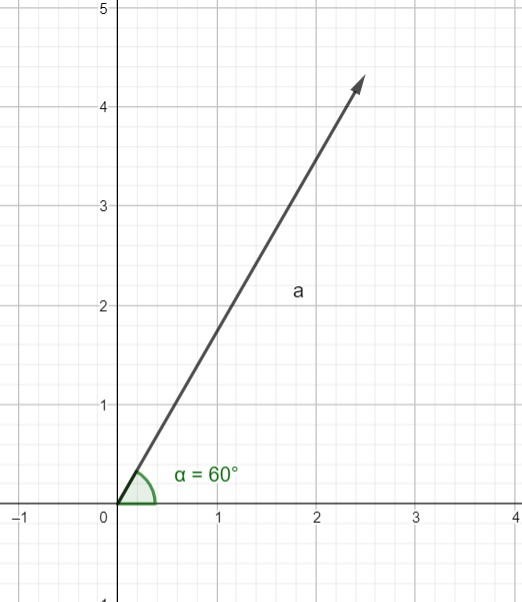
\includegraphics[width = 6cm]{Opgave_21-30/Opgave_22/22.jpg}
\newpage
\subsection{Opgave 23}

En vektor $\Vec{c}$ har længden 6 og retningsvinklen $127^{\circ}$\\\\
Bestem koordinaterne for $\Vec{c}$.\\\\

\ans
For at bestemme vektor c's koordinaterne gør vi bruge af følgende formel
\begin{align*}
    \Vec{c} = \begin{pmatrix}l\cdot \cos(v) \\ l\cdot \sin(v)\end{pmatrix}
\end{align*}
Her er l vektorens længde og v er vektorens retningsvinkel. Indsætter vi de givne værdier får vi
\begin{align*}
    \Vec{c} = \begin{pmatrix}6\cdot \cos(127^{\circ}) \\ 6\cdot \sin(127^{\circ})\end{pmatrix} = \begin{pmatrix}-3.61 \\ 4.79\end{pmatrix}
\end{align*}
Vektoren er illustreret nedenfor\\\\
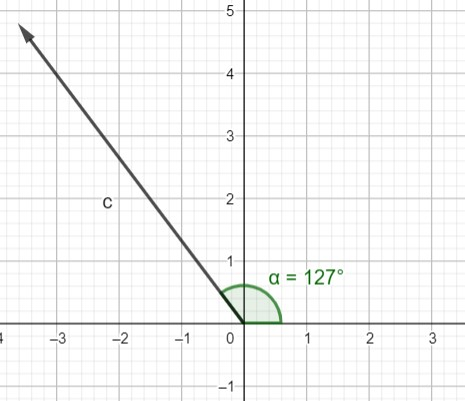
\includegraphics[width = 6cm]{Opgave_21-30/Opgave_23/23.jpg}
\newpage
\subsection{Opgave 24}

På figuren nedenfor ses repræsentanter for vektorerne $\vec{a}$, $\vec{b}$ og $\vec{c}$.

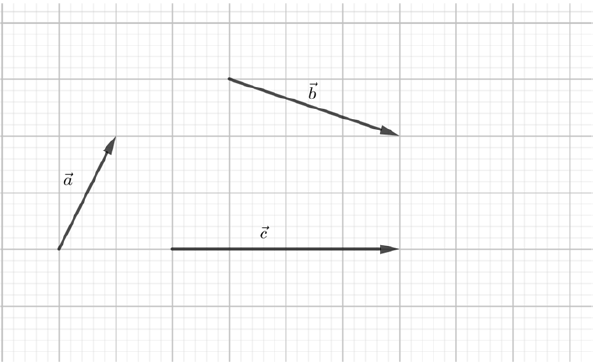
\includegraphics[width = 0.5\textwidth]{Opgave_21-30/Opgave_24/24.png}

Indtegn en repræsentant for vektoren $\vec{a} + \vec{b} + \vec{c}$.

\ans

Først aflæser vi vektorernes x og y komponenter. X komponenten af en vektor er hvor meget vi går hen ad x - aksen, og y komponent er hvor meget vi går op ad y aksen. Nedenstående figur illustrerer hvordan man kan aflæse en vektors x og y komponenter ud fra figuren. 

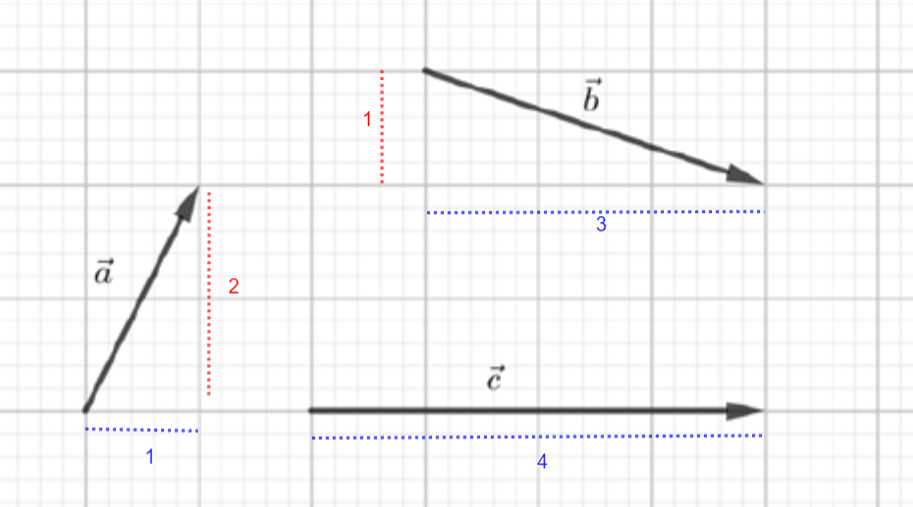
\includegraphics[width = 0.5\textwidth]{Opgave_21-30/Opgave_24/24.1.png}

De blå linjer er vektorernes x komponenter og de røde linjer er vektorernes y komponenter.

Vi har nu
\begin{align*}
    \Vec{a} &= \begin{pmatrix} 1 \\ 2 \end{pmatrix}\\
    \Vec{b} &= \begin{pmatrix} 3 \\ -1 \end{pmatrix}\\
    \Vec{c} &= \begin{pmatrix} 4 \\ 0 \end{pmatrix}
\end{align*}

Vi kan nu beregne summen af de 3 vektorer
\begin{align*}
    \Vec{a} + \Vec{b} + \Vec{c} = \begin{pmatrix} 1 \\ 2 \end{pmatrix} + \begin{pmatrix} 3 \\ -1 \end{pmatrix} + \begin{pmatrix} 4 \\ 0 \end{pmatrix} = \begin{pmatrix}
        1 + 3 + 4 \\ 2 - 1 + 0
    \end{pmatrix}  = \begin{pmatrix}
        8 \\ 1
    \end{pmatrix}
\end{align*}

Nu indtegner vi vektoren $\begin{pmatrix}
    8 \\ 1
\end{pmatrix}$
ind i et koordinatsystem. 

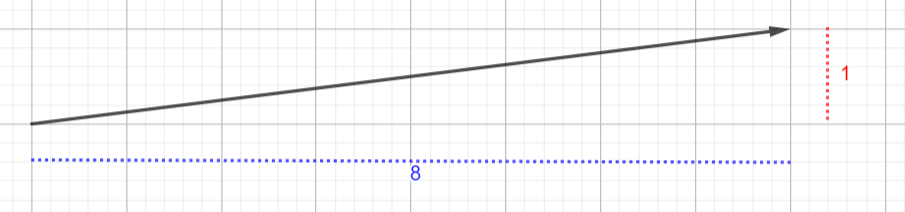
\includegraphics[width = 0.5\textwidth]{Opgave_21-30/Opgave_24/24.2.png}


\end{document}